%%%%%%%%%%%%%%%%%%%%%%%%%%%%%%%%%%%%%%%%%
% Short Sectioned Assignment
% LaTeX Template
% Version 1.0 (5/5/12)
%
% This template has been downloaded from:
% http://www.LaTeXTemplates.com
%
% Original author:
% Frits Wenneker (http://www.howtotex.com)
%
% License:
% CC BY-NC-SA 3.0 (http://creativecommons.org/licenses/by-nc-sa/3.0/)
%
%%%%%%%%%%%%%%%%%%%%%%%%%%%%%%%%%%%%%%%%%

%----------------------------------------------------------------------------------------
%	PACKAGES AND OTHER DOCUMENT CONFIGURATIONS
%----------------------------------------------------------------------------------------

\documentclass[paper=letter, fontsize=11pt]{scrartcl} % A4 paper and 11pt font size

\usepackage[T1]{fontenc} % Use 8-bit encoding that has 256 glyphs
\usepackage{fourier} % Use the Adobe Utopia font for the document - comment this line to return to the LaTeX default
\usepackage[english]{babel} % English language/hyphenation
\usepackage{amsmath,amsfonts,amsthm} % Math packages
\usepackage{graphicx}
\usepackage{lipsum} % Used for inserting dummy 'Lorem ipsum' text into the template
\usepackage{hyperref}

\usepackage{sectsty} % Allows customizing section commands
\allsectionsfont{\centering \normalfont\scshape} % Make all sections centered, the default font and small caps

\usepackage{fancyhdr} % Custom headers and footers
\pagestyle{fancyplain} % Makes all pages in the document conform to the custom headers and footers
\fancyhead{} % No page header - if you want one, create it in the same way as the footers below
\fancyfoot[L]{} % Empty left footer
\fancyfoot[C]{} % Empty center footer
\fancyfoot[R]{\thepage} % Page numbering for right footer
\renewcommand{\headrulewidth}{0pt} % Remove header underlines
\renewcommand{\footrulewidth}{0pt} % Remove footer underlines
\setlength{\headheight}{13.6pt} % Customize the height of the header

\numberwithin{equation}{section} % Number equations within sections (i.e. 1.1, 1.2, 2.1, 2.2 instead of 1, 2, 3, 4)
\numberwithin{figure}{section} % Number figures within sections (i.e. 1.1, 1.2, 2.1, 2.2 instead of 1, 2, 3, 4)
\numberwithin{table}{section} % Number tables within sections (i.e. 1.1, 1.2, 2.1, 2.2 instead of 1, 2, 3, 4)

\setlength\parindent{0pt} % Removes all indentation from paragraphs - comment this line for an assignment with lots of text

%----------------------------------------------------------------------------------------
%	TITLE SECTION
%----------------------------------------------------------------------------------------

\newcommand{\horrule}[1]{\rule{\linewidth}{#1}} % Create horizontal rule command with 1 argument of height

\title{	
\normalfont \normalsize 
\textsc{University of California Irvine} \\  % Your university, school and/or department name(s)
\textsc{Course: Introduction to Digital Logic Lab (31L) Summer 2015} \\ [25pt]
\horrule{0.5pt} \\[0.4cm] % Thin top horizontal rule
\huge Lab 0 report\\ % The assignment title
\horrule{2pt} \\[0.5cm] % Thick bottom horizontal rule
}

\author{Ashkan Eghbal \\ Student ID: 12345678} % Your name


\date{\normalsize\today} % Today's date or a custom date

\begin{document}

\maketitle % Print the title

%----------------------------------------------------------------------------------------
%	PROBLEM 1
%----------------------------------------------------------------------------------------

\section{Latex installation and tutorial}

Latex is a high-quality document preparation system. In order to set it up on your Windows machine you need to download and install some tools which are discussed in the following Section. However, there are hundreds of tools that you can use to set up Latex and this tutorial is one of them. 

%------------------------------------------------

\subsection{Tools} %Heading on level 2 (subsection)

To set up a latex system on your computer you need two major programs to be installed. The first one is the latex engine and the second one is the text editor that you can use. You also need a tool to show the output of your Latex project which is usually a ".pdf"' file. 

%------------------------------------------------

\subsubsection{Latex engine} %Heading on level 3 (subsubsection)

You can use MiKTeX as a free Text distribution for Windows systems. Once you reach the \href{http://miktex.org/download} {\textit{website}}, then press on download tab which directs you to installation file download link. Run the file once it is downloaded. The installation wizard of MiKTeX will now pop up. 

\subsubsection{Latex text editor}
As discussed earlier there are many free text editors for Latex too. The TeXnicCenter is chosen here as one of them that you can \href{http://www.texniccenter.org/download/}{\textit{download}} it from here.

\subsubsection{}
You can use any pdf reader file including acrobat reader, but the \href{http://www.pdflite.com/}{\textit{PDFlite}} which is a free pdf reader and writer tool. It  is a perfect match for TeXnicCenter tool. One of the benefit of PDFlite comparing to acrobat application is that every time you edit your report there is no need to close the pdf file and run the project. It automatically update the pdf file after you run the project in TeXnicCenter


\section{Lists}

%------------------------------------------------
% to add a list to your report

In case you want to have bullet list you can use the following format. If you want to have numerical lists refer to Section~\ref{sec:general_notes}.
\subsection{Example of list (3*itemize)}
\begin{itemize}
	\item First item in a list 
		\begin{itemize}
		\item First item in a list 
			\begin{itemize}
			\item First item in a list 
			\item Second item in a list 
			\end{itemize}
		\item Second item in a list 
		\end{itemize}
	\item Second item in a list 
\end{itemize}

%-----------------------------------------------
% to add a table
\section{Example of tables}
You can easily use this code to add a table to your report. There are many options for tables that you can easily find them on line through the wiki pages for latex table related commands.
\begin{table}[h]
\centering
\caption{Truth table of AND gate}
\label{my-label}
\begin{tabular}{|c|c||c|}
\hline
\textbf{Input1} & \textbf{Input0} & \textbf{Output}    \\
\hline 
0&0  &0    \\
\hline
 0&1  &0    \\
\hline
 1&0  & 0 \\
\hline
1&1 &1  \\
\hline
\end{tabular}
\end{table}


%------------------------------------------------
%to add a figure:
\section{Example of figures}

You can easily use this code to add a figure to your report.
\begin{figure}[ht]
	\caption{TeXnicCenter viewer tab configuration}
	\centering
			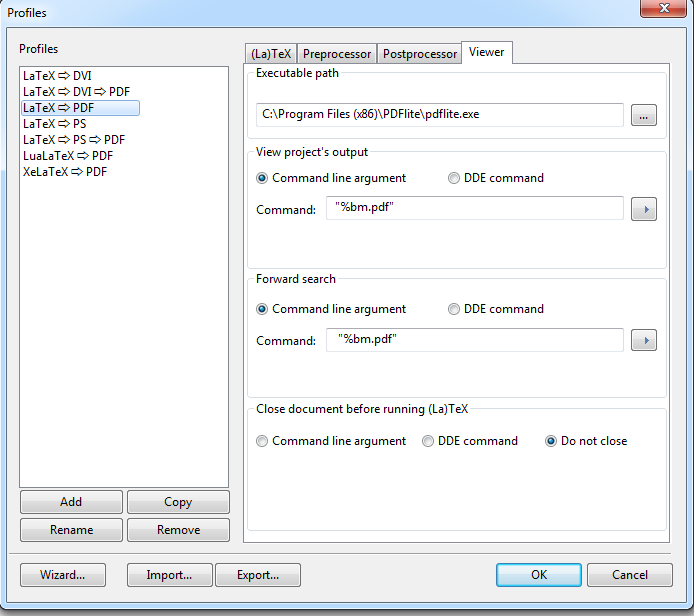
\includegraphics[width=0.7\textwidth]{figs/pdfliteviewer.png} %to change the size of figure modify the 0.7 value
	\label{fig:pdflite_viewer_config} %use inside {} inside \ref{} command to refer this figure in your text. For example: figure~\ref{fig:pdflite_viewer_config}
\end{figure}

%\begin{figure}[hb]
	%\caption{UCI-logo}
	%\centering
			%\includegraphics[width=0.4\textwidth]{figs/uci.png} %to change the size of figure modify the value of 0.4
				%\label{fig:uci}
%\end{figure}




\section{General notes}
\label{sec:general_notes}
Besides considering note you can find the format of numerical list in this section.
\begin{enumerate}
\item Make sure to install your Latex engine first and then install the Latex text editor (TeXnicCenter). So first install MikteX and then TeXnicCenter.
\item Once you have installed both you only need to click on the icon of TeXnicCenter. When you run it for the first time, the configuration wizard window shows ups. In this step you may be asked to choose the Distribution directory. In this case you need to locate the path in which the installed MikTeX on your computer. 		This address by default is in $C:  . . . \backslash programfiles \backslash MikTeX2.9 \backslash miktex \backslash bin$
	\begin {enumerate}
	\item \textit{2.9} in this path is the version of your MikTeX which can be different based on the version you have downloaded.
	\end {enumerate}
\item In configuration wizard window make sure to choose your favorite pdf viewer full path. 
\item If you have forgotten to choose your favorite application during installation you can access to it by choosing \textit{Build} tab and then \textit{Define Output Profiles} option.
	\begin {enumerate}
	\item Go to Build->Define Output Profiles-> choose "Latex => PDF"
	\item Then choose viewer tab on the right window
	\item If you want to use PDFlite as your viewer here is the setting and commands (as shown in figure~\ref{fig:pdflite_viewer_config})
	\begin {enumerate}
	\item Executable path should be the location of pdflite file in the directory you have installed PDFlite software. It should be something like
	
	$C: . . . \backslash Program Files (x86) \backslash  PDFlite \backslash  pdflite.exe$
	\item For both \textit{View Projects Output} and \textit{Forward search}, choose Command line argument option and add the following command
	$"\%bm.pdf"$
	\item Finally choose \textit{Do not close} option too.
	\end {enumerate}
	\item If you have chosen Adobe acrobat
		\begin{enumerate}
		\item Go to Build->Define Output Profiles-> choose "Latex => PDF"
		\item In the viewer tab, change the executable location to point to
		
			$C:... \backslash Program Files  \backslash Adobe \backslash Reader 10.0 \backslash Reader \backslash AcroRd32.exe$
			\item	In View project's output and Forward search : Select DDE command and enter
			
			 $[DocOpen("\%bm.pdf")][FileOpen("\%bm.pdf")]$ 
			
			 $Server: arcroviewR10$ ~~~~  $Topic: Control$
		\end{enumerate}
	\end {enumerate}
\item To write your project, double click on the file with \textit{.tcp} extension to open the project. If you cannot see the extension of your files:
	\begin{enumerate}
		\item Go to start or in Windows 8 press the start button
		\item Type Folder Options and press on it
		\item Under View tab, deselect \textit{Hide extensions for known files types.}
	\end {enumerate}

\item Do not forget to update the assignment number and your name and student ID. The date will be generated automatically.
\item To compile your report you need to make sure on top Latex => PDF is chosen in a drop down list	
\item Then press F7 or press on the first button right side of Latex => PDF option, which is called Build Output;  then make sure there is no error which is reported in Build output window.
\item To check the output, you only need to press on F5 only first time you have opened the project. If there is no problem the output of your file should be opened through the PDF viewer application you have chosen.
\item If you are using PDFlite as viewer there is no need to press F5 after compiling your code after the first time. You can see your modifications by only compiling the project in PDFLite if there is no error in your project.
\item For more options and command check the \href{https://en.wikibooks.org/wiki/LaTeX}{\textit{Latex wiki page}}.
\end{enumerate}

%\begin{figure}[h]
	%\caption{UCI-logo}
	%\centering
			%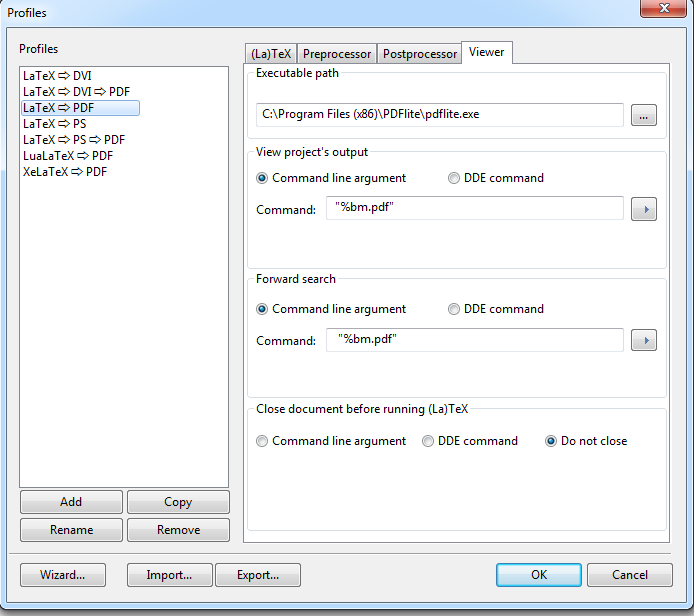
\includegraphics[width=0.9\textwidth]{figs/pdfliteviewer.png} %to change the size of figure modify the value of 0.4
	%\label{fig:pdflite_latex_config}
%\end{figure}



%----------------------------------------------------------------------------------------



%----------------------------------------------------------------------------------------


\end{document}